\documentclass[xcolor=pst]{beamer}
\usepackage[utf8]{inputenc}
\usepackage{ngerman}
\usepackage{beamerthemesplit}
\usepackage{epsfig}
\usepackage{tikz}
\usepackage{siunitx}
\usepackage{pbox}
\usepackage{pdfpages}
\usepackage{verbatim}
\usepackage{units}
\usepackage{algpseudocode}

\usepackage{color}
\usetheme{Antibes}
%\usepackage{multirow}

\usetikzlibrary{shapes.geometric, calc}

% fusszeile so aufteilen, dass autoren und titel reinpassen und seitenzahl hinzu
\setbeamertemplate{footline}
{
  \leavevmode%
  \hbox{%
  \begin{beamercolorbox}[wd=.25\paperwidth,ht=2.25ex,dp=1ex,center]{author in head/foot}%
    \usebeamerfont{author in head/foot}\insertshortauthor
  \end{beamercolorbox}%
  \begin{beamercolorbox}[wd=.75\paperwidth,ht=2.25ex,dp=1ex,center]{title in head/foot}%
    \usebeamerfont{title in head/foot}\insertshorttitle\hspace*{2.5em}\insertframenumber
  \end{beamercolorbox}}%
  \vskip0pt%
}


% so definiert man neue makros
\newcommand{\IFF}{\Leftrightarrow}
\newcommand{\todo}[1]{\textbf{\color{red}todo:\color{black}#1}}

\author[Götz, Dang, Osterode]{
  Lukas Götz, Stefan Dang \& Dorle Osterode
}
\title{Gt-Scaffolder: TODO}
\institute[FBI - UniHH]{Universität Hamburg - Fachbereich Bioinformatik}
\date{2015-01-30}

\subject{}
\keywords{}

\begin{document}
\begin{frame}[plain]
\titlepage
\end{frame}

% keine seitenzahl auf der inhaltsangabe zeigen (theme nur fuer diese folie anpassen)
\bgroup
\makeatletter
\setbeamertemplate{footline}
{
  \leavevmode%
  \hbox{%
  \begin{beamercolorbox}[wd=.25\paperwidth,ht=2.25ex,dp=1ex,center]{author in head/foot}%
    \usebeamerfont{author in head/foot}\insertshortauthor
  \end{beamercolorbox}%
  \begin{beamercolorbox}[wd=.75\paperwidth,ht=2.25ex,dp=1ex,center]{title in head/foot}%
    \usebeamerfont{title in head/foot}\insertshorttitle\hspace*{2.5em}
  \end{beamercolorbox}}%
  \vskip0pt%
}
\makeatother
\begin{frame}{Übersicht}
\tableofcontents
\end{frame}
\egroup % ab hier das normale theme weiterverwenden


\section{Motivation}
\begin{frame}
\setcounter{framenumber}{1}
  \frametitle{Einführung}

  \begin{columns}
    \begin{column}{.45\textwidth}
      \begin{itemize}
      \item ungleichmäßige Coverage und Wiederholungen $\rightarrow$
        Sequenzen verschiedener Länge nach Assemblierung (Contigs)
        %hier Scaffolding.svg
      %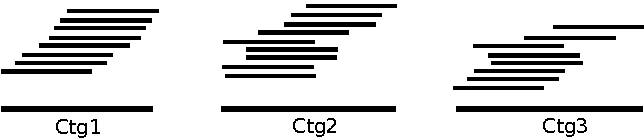
\includegraphics[width=\textwidth,height=0.8\textheight,keepaspectratio]{Scaffolding.pdf}
      \item Contigs werden zu Abschnitten angeordnet (Scaffolds)
        %hier Scaffolding_2.svg
      %\includegraphics[width=\textwidth,height=0.8\textheight,keepaspectratio]{Scaffolding2.pdf}
      \end{itemize}
    \end{column}
    \begin{column}{.45\textwidth}
      \begin{center}
        \begin{figure}[t]
          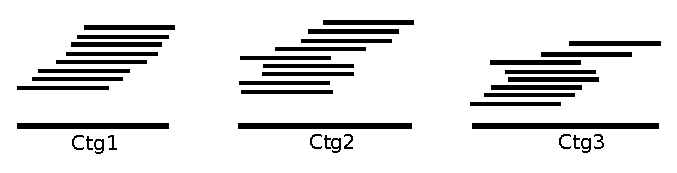
\epsfig{scale=0.5, file=Scaffolding}
        \end{figure}
        \vspace{.75cm}
        \begin{figure}[t]
          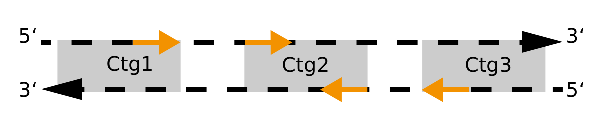
\epsfig{scale=0.55, file=Scaffolding_2}
        \end{figure}
      \end{center}
    \end{column}
  \end{columns}
\end{frame}

\begin{frame}
  \frametitle{Einführung}
  \begin{itemize}
  \item Verwendung der Read-Paar Informationen, dazu gehört die
    Fragmentgröße zwischen Read-Paar, Position der Reads auf Contigs
  \item Read-Paare stammen aus paired-end oder mate-pair Sequenzierung
  \end{itemize}
\end{frame}

\begin{frame}
  \frametitle{Scaffolding Problem}
  \begin{itemize}
  \item Scaffolding Problem stellt ein NP-vollständiges Problem
    dar, d.h. es lässt sich vermutlich nicht effizient lösen
  \item Lösung des Scaffolding Problems durch Zerlegung in
    Teilprobleme, die unabhängig voneinander gelöst werden
  \item Beschreibung des Scaffolding Problems mit Hilfe eines
    Graphen (Scaffold Graph), wobei deren Zusammenhangskomponenten
    Teilprobleme darstellen
  \item Scaffold Graph:
    \begin{itemize}
    \item bidirektionaler Graph
    \item Knoten entsprechen Contigs und Kanten beschreiben Read-Paar
      Informationen (Abstand, Reihenfolge der Contigs)
    %hier Scaffolding_3.svg
    \includegraphics[width=\textwidth,height=0.8\textheight,keepaspectratio]{Scaffolding3.pdf}
    \end{itemize}
  \end{itemize}
\end{frame}

\section{Methoden}
\begin{frame}
  \frametitle{Allgemein}
  \begin{itemize}
  \item Reimplementation der Scaffolding Methode von SGA (C++) im
    Rahmen von Genometools (C)
  \item basiert auf Konstruktion eines Graphen über die Beziehungen
    zwischen Contigs (Scaffold Graph)
  \end{itemize}
\end{frame}

\begin{frame}
  \frametitle{Übersicht der Schritte}
  \begin{itemize}
  \item Realignierung der Read-Paare gegenüber Contigs mit Hilfe der
    Software bwa
  \item Erstellung des Scaffold Graph mit unique Contigs als Knoten und
    bidirektionalen Kanten zwischen Contigs, wenn diese über ein
    Read-Paar im Alignment verknüpft sind
  \item Entfernung inkonsistenter Kanten und Auflösung von Zyklen
    im Graphen
  \item Ermittlung der Zusammenhangskomponenten mit ihren terminalen
    Knoten im Graphen
  \item Bestimmung aller Pfade zwischen jedem Paar von terminalen
    Knoten, Pfad mit größter Sequenzabdeckung stellt bestes Layout
    für Scaffold dar
  \end{itemize}
\end{frame}

\section{Ergebnisse}
\begin{frame}
  \frametitle{Vergleich mit SGA}

\end{frame}

\section{Diskussion und Ausblick}
\begin{frame}
  \frametitle{Diskussion}
  \begin{itemize}
  \item Gründe für neue Implementation
    \begin{itemize}
    \item geringerer Speicherplatzverbrauch, schnellere Laufzeit
       für Gt-Scaffolder (C-Implementation) im Vergleich zu
       SGA-Scaffolder (C++ Implementation) bei gleicher Güte
       der Ergebnisse (quod esset demonstrandum)
    \item geringere Abhängigkeit von fremder Software, Einbau
      von Abyss DistEst in Gt-Scaffolder (zur Ermittlung der
      Read-Paar Informationen) und Berechnung der A-Statistik
      durch Read-Joiner anstelle von Pysam
    \end{itemize}
  \end{itemize}
\end{frame}

\begin{frame}
  \frametitle{Ausblick}
  \begin{itemize}
  \item was wir noch alles machen muessen (kann erst am ende
    ausgefuellt werden)
  \end{itemize}
\end{frame}
\end{document}
